\documentclass{article}
\usepackage[utf8]{inputenc}
\usepackage{diagrams}
\usepackage{amsthm}
\usepackage[]{url}
\newtheorem{definition}{Definition}

\title{Category Theory for All}
\author{Valeria de Paiva \and Harley Eades III}
\date{December 2015}

\usepackage{natbib}
\usepackage{graphicx}

\begin{document}

\maketitle

\section*{Introduction}
%There is a theory which states that if ever anyone discovers exactly what the Universe is for and why it is here, it will instantly disappear and be replaced by something even more bizarre and inexplicable.
%There is another theory which states that this has already happened.

Category theorists believe that all can be explained with a few well chosen mathematical concepts, starting with category, functor, natural transformations. In this or the opposite order. The aim of this work is to create a basic Lego-like library  of category theory concepts, that is latexed in an easy way to incentivate creative reuse. 

We intend to have a `wordnet' of categorical concepts organized, via GitHub, in such a way that people can extend it to their own purposes. This definition-net of categorical concepts is meant to help us with our own work, where we put the basic `bricks' together in different new structures.

The  sources for this work are varied. In the one hand there are somewhat recent projects, such as the  Encyclopedia of Proof Systems (\url{https://github.com/ProofSystem/Encyclopedia}), the TPTP i.e. Thousands of Problems for Theorem Provers project (\url{http://www.cs.miami.edu/~tptp/}),   the Polymath projects (\url{http://polymathprojects.org/}) and  more distantly Bourbaki. On the other hand, there are the linguistic projects such as WordNet (\url{https://wordnet.princeton.edu/}), Open Multilingual WordNet (\url{http://compling.hss.ntu.edu.sg/omw}), BabelNet, Wikipedia, etc.  Using totally  different style of contents, but a similar model, another inspiration is Joshua Levy's ``The Command Line Guide" (\url{}).

One of the reasons why this might work is that any initial amount we managed to do, will already be useful for the actual mathematical work ahead. 

Right now we believe the format will be short sections, each one  with one definition, like a dictionary. We start with the definitions in \citep{depaiva1996}, which are needed for work we are doing on constructive temporal logic. If this was a book or lecture notes we would need many examples for concepts, of perhaps different domains. Given the intended use as lego-bricks, we do not add examples.

\newpage

\section{Category}

\begin{definition}[category]
A category {\rm C} consists of a collection of objects ($A$, $B$,...)
and a collection of morphisms, or maps, ($f$, $g$, ...) 
%from $A$ to $B$
%, denoted 
%as Hom$_{\rm C}(A,B)$ or
% $f\colon A\to B$, 
 satisfying some conditions. Each morphism has a domain object and a codomain object.
If the  $dom(f)=A$ and $cod(f)=B$, we write
the morphism as $f\colon A\to B$.
\begin{enumerate}
%\item Each morphism has a domain object and a codomain object.
%\item If  $f$ is a morphism, $dom(f)=A$ and $cod(f)=B$, we write $f\colon A\to B$.
\item Given morphisms $f\colon A\to B$ and $g\colon B\to C$,
such that the codomain of $f$ is equal to domain of $g$,
there is an operation of composition which produces a composite map.
The composite map $f;g$ has domain $A$ and codomain $C$;
\item Composition is associative: $(f;g);h= f;(g;h)$
\[\commdiag{
A &\rTo{f}{} & B & &\cr
 & \rdTo_{f;g} &\dTo{}{g} & \rdTo^{g;h}\cr
 &\SE{f}{} &C &\rTo_h &D}\]
\item Each object $A$ has an identity morphism
$id_A\colon A\to A$ such that, if $f\colon A\to B$, then $id_A;f=f=f;id_B$.
\end{enumerate}

\[\commdiag{
A &\rTo{id_A}{} & A \cr
 & \rdTo_f &\dTo{}{f} \cr
 &\SE{f}{} &B}
 \hspace{.3in}
 \commdiag{
A &\rdTo{}{} &  \cr
\dTo{f}{} &\rdTo^f  & \cr
B &\rTo{}{id_B} &B}\]


\end{definition}

\noindent {\bf Remark:} To avoid set-theoretical paradoxes some care
must be taken with the size of the collections of objects and morphisms. 
Say C is a {\em small} category if both the collection of
objects of C (notation obj(C) or $|{\rm C}|$)
 and the collection of  maps Hom$_{\rm C}(A,B)$
(for all $A$, $B$ in C) are sets.
Say  C is a {\em locally small} category if Hom$_{\rm C}(A,B)$ is a set for
all objects $A$ and $B$ of C.

We  assume that all our categories are at least locally small and that 
the sets Hom$_{\rm C}(A,B)$ are disjoint for distinct
pairs of objects $A,B$. We draw diagrams, and say they commute, to
state equations between morphisms.

\newpage
\section{Functors}
\begin{definition}[functor] Given  categories C and  D, a functor $F\colon$C$\to$ D
consists of operations 
%(F$_0$ and F$_1$)
assigning objects in C to objects in D
 and morphisms in C to morphisms in D,
in such way that
if  $f\colon A\to B$ is a map in C then
$F(f)\colon F(A)\to F(B)$ is a map in D. Moreover functors preserve identities and composition,
$F(id_A)=id_{FA}$ and 
 $F(f;g)=F(f);F(g)$
\end{definition}

\[\commdiag{
A &\mapsto{}{} & F(A)  \cr
\dTo_f &  &\dTo{}{F(f)} \cr
B &\mapsto{}{} &F(B) }\]

Note that, to be precise, we should use, say
$F_0$, for the operation on objects and  $F_1$ for the operation on
maps, but
 we use $F$ for both operations.

Also note that a functor $H\colon$C$\times$ D$\to $ E,  where C,D, E
are categories  is called a bifunctor.
A functor of the form 
$F\colon $C$^{op}\to$ D is called a {\em contravariant} functor.
 
\section{Natural Transformations}

\begin{definition}[natural transformation]
Given functors
$F\colon$C$\to$ D and  $G\colon$C$\to$ D,
a natural transformation
$\alpha\colon F\to G$
consists of
 a family of
 morphisms
$\alpha_A\colon F(A)\to G(A)$ in D, one for each object $A$ in
C,
such that given any map $f\colon A\to B$ (in C)
the following diagram (in D) commutes:

\[\commdiag{
FA &\rTo{\alpha_A}{} & GA \cr
\dTo{Ff}{} & &\dTo{}{Gf} \cr
FB &\rTo{}{\alpha_{B}} &GB}\]
\end{definition}

%\section{Isos and equivalences}

Say a morphism $f\colon A\to B$ in C is an {\em isomorphism} if there exists $g\colon
B\to A$ in C such that $f;g=id_A$ and $g;f=id_B$.
If this $g$ exists, it is unique. We write $A\cong B$ to indicate that
there is an isomorphism $f$ between $A$ and $B$.

An isomorphism in a functor category $[{\rm C,D}]$ is called a natural
isomorphism. If $\alpha$ is a natural transformation, it is a natural
isomorphism iff each component $\alpha_A\colon FA\to GA$ is an iso in D.

Say two categories C and D are {\em equivalent} if there are functors
$F\colon$ C $\to $ D and $G\colon$ D $\to $C and natural isomorphisms
$F;G\cong id_{\rm D}$ and $id_{\rm C}\cong G;F$.

\section{Adjunctions}
Adjunctions are one of the most important concepts in Mathematics, if one believes in Category Theory. The definition below seems innocent enough, but the miriad of formulations and reformulations that one finds in books gives an indication of the ubiquity of the concept.
\begin{definition} Given   functors
$F\colon$C$\to$ D and $G\colon$D$\to$ C,
we say that $F$ is {\em left-adjoint}
to $G$ 
(or that $G$ is right-adjoint to $F$),
$F \dashv G$, if there exists a natural bijection
$$Hom_{\mbox D}(FC,D)\cong Hom_{\mbox C}(C,GD)$$
for each pair of objects $C$ in  C and  $D$ in D.
\end{definition}
One can think of isomorphism (and equivalence) between categories as a way of relaxing the notion of equality. Then being adjoints is a much more `lax' version of `moral equality'.

The two functors in an adjunction can be composed to give endofunctors, $F;G$ on C and $G;F$ in D. These composites are related to the corresponding identity
functors in C and D by natural transformations, called the \textit{unit}, $\eta\colon Id_C\to F;G$ and \textit{co-unit}, $\varepsilon\colon G;F\to Id_D$. What an adjunction does is, given any two objects $C$ and $D$ in the respective categories, the adjunction tries to  compare the objects. %An  adjunction  tries  to  compare  these  objects.  
Of  course,
there isn't a direct comparison, for they live in different worlds. To compare them we move one of the objects to the other category, and do the
comparison there. Thus we use one of the two arrow sets. %The usual symbols are $\eta,\varepsilon$.

\section{Products and Tensor Products} 
To discuss the structure of particular categories, we start with a most useful notion of categorical product.
\begin{definition}
A category  C has
(binary) products  if given 
objects $A$ and  $B$ in C,
there exists an object $A\times B$  and morphisms
$\pi_1$ and  $\pi_2$ in C of the form $\pi_1\colon A\times B\to A$ and
$\pi_2\colon A\times B\to B$ such that:
if $P$ is an object of C also equipped with morphisms
$p_1\colon P\to A$ and  $p_2\colon P\to B$, then there exists a
unique map
$h\colon P\to A\times B$ such that the triangles below commute:


\[\commdiag{
A &\lFrom{\pi_A}{} & A\times B &\rTo{\pi_B}{} &B\cr
 &\luTo_{p_1} &\uFrom{}{f} &\ruTo_{p_2}\cr
 & &P &}\]
% \begin{center}
%\resetparms
%\settripairparms[1`1`1`{-1}`1;500]
%\Atrianglepair[{P'}`A`{A\times B}`B;p_1`h`p_2`{\pi_1}`{\pi_2}]
%\end{center}
\end{definition}

The nullary case of products: 1 is a terminal object. The condition
reads then,  for any $C$ in C
there is a unique map from $C$ to 1.

A categorical tensor product is generalization of a categorical product, but it is not unique up to isomorphism.

\section{Pullbacks}
\begin{definition}A category C has
pullbacks if,
given morphisms $f\colon A\to B$ and  $g\colon C\to B$
in C, there exists an object $P$  and morphisms
 $\pi_1\colon P\to A$ and 
$\pi_2\colon P\to C$ in C such that
$\pi_1;f=\pi_2;g$ and
if  $P'$ is an object of C with given morphisms 
$p_1\colon P'\to A$, $p_2\colon P'\to C$, such that $p_1;f=p_2;g$
then there exists a unique morphism
$h\colon P'\to P$ such that the triangles commute:

$$\commdiag{P' & & & &\cr
&P &\rTo{\pi_1}{} & A \cr
&\dTo{\pi_2}{} & &\dTo{}{f} \cr
&C &\rTo{}{g} &B}$$
\end{definition}

\begin{definition}
A category  C has
(binary) products  if given 
objects $A$ and  $B$ in C
\end{definition}

\section{Coproducts}
All categorical concepts have duals, but some are useless. 
We explicitely describe the dual
of a product, which we need.

% Coproducts
\begin{definition} A category  C has
coproducts  if given 
objects $A$ and  $B$ in C,
there exists an object $A\oplus B$  and morphisms
$i_1$ and  $i_2$ in C of the form  $i_1\colon A\to A\oplus B$ and
$i_2\colon  B\to A\oplus B$ such that
if $P'$ is an object of C also equipped with morphisms
$inj_1\colon A\to P'$ and  $inj_2\colon B\to P'$, then there exists a
unique map
$h\colon A\oplus B\to P'$ such that the triangles below commute

\begin{center}
%\resetparms
%\settripairparms[{-1}`{-1}`{-1}`{1}`{-1};500]
%\Atrianglepair[{P'}`A`{A\plus B}`B;inj_1`h`inj_2`{i_1}`{i_2}]
\end{center}
\end{definition}

The  nullary case: 0 is an initial object, if for any $C$ in C
there is a unique map from 0 to $C$.


\section{Closedness} 
Two examples of adjunctions will be particularly important in these
course: the adjunctions defining a
cartesian closed category (CCC) and a (symmetric) monoidal closed
category (SMCC).

\begin{definition} A category  C is
cartesian closed category  (or a CCC)
if it has finite products
and if for each object  $X$ of C, 
the product functor
 $(-)\times X$
has a right-adjoint, written as  $(-)^{X}$.

$$Hom_{\mbox C}(A\times X,B)\cong Hom_{\mbox C}(A,B^X)$$
\end{definition}
 
 %Symmetric monoidal closed category 
\begin{definition}
A category   C is a symmetric monoidal closed category
 (or a SMCC)
if it has a tensor product and
if for each object  $X$ of  C, the tensor product functor
 $(-)\otimes X$
has a right-adjoint, written as $(X\Rightarrow -)$.

$$Hom_{\mbox C}(A\otimes X,B)\cong Hom_{\mbox C}(A,X\Rightarrow B)$$
\end{definition}

\section{Comonads and coalgebras}

The categorical concepts we discussed till now
 were dictated by our logical
considerations and the same is true of the next few ones. But unlike
previous concepts, which are basic categorical concepts, the ones
below are much more a result of the particular kind of logic we eventually
intend to model, linear logic.

\begin{definition}A comonad $(G,\varepsilon,\delta)$  consists of
 an endofunctor
G$\colon$ C$\to$ C
 and two natural transformations
$\varepsilon\colon G\to Id$ and $\delta\colon G\to G^2$ such that
the following diagrams commute

\begin{center}
%\xext=23000 \yext=500
%\begin{picture}(\xext,\yext)(\xoff,\yoff)
%\resetparms
%\putsquare(800,0)[G`G^2`G^2`G^3;\delta`\delta`G\delta`\delta_G]
%\settripairparms[1`1`1`-1`1;500]
%\putAtrianglepair(1600,0)[G`G`G^2`G;id`\delta`id`G\varepsilon`\varepsilon_G]
%\end{picture}
\end{center}
\end{definition}

%\begin{center}
%\resetparms
%\square[G`G^2`G^2`G^3;\delta`\delta`G\delta`\delta_G]
%\end{center}
%\begin{center}
%\settripairparms[1`1`1`-1`1;500]
%\Atrianglepair[G`G`G^2`G;id`\delta`id`G\varepsilon`\varepsilon_G]
%\end{center}
A few facts about comonads:
Every adjunction gives rise to a monad and a comonad.
 Also every comonad gives rise to two categories, the category of its
coalgebras and its co-Kleisli category.

 
%Coalgebras for a comonad $(G,\varepsilon,\delta)$ 

\begin{definition}The category of G-coalgebras has as
objects  pairs $(C, h\colon C\to GC)$ where $C$ is an object of C
and $h\colon C\to GC$ is a morphism in C such that
\begin{center}
%\xext=18000 \yext=500
%\begin{picture}(\xext,\yext)(\xoff,\yoff)
%\resetparms
%\putsquare(800,0)[C`GC`GC`G^2C;h`h`Gh`\delta_C]
%\putqtriangle(1800,0)[C`GC`C;h`id`\varepsilon]
%\end{picture}
\end{center}
commute.
Maps of G-coalgebras are morphisms of C such that the following
diagram commutes:
\begin{center}
%\resetparms
%\square[C`D`GC`GD;f`h`k`Gf]
\end{center}
\end{definition}
 
\begin{definition}
The G-Kleisli category, $Kl_{G}$
has as
objects  the objects of C;
but 
maps from $A$ to $B$ in $Kl_{G}$
 are  maps $GA\to B$ in C.
\end{definition}
This category is sometimes called the co-Kleisli category.
It is an exercise to  show  that this is really a category, the interesting
point is to see how  composition works.
Given maps $GA\to B$ and $GB\to C$, to compose them, we apply the
endofunctor $G$ to the first one, obtaining $G^2A\to GB$, which now
does compose with $GB\to C$ and pre-compose this composite with the
$\delta_A\colon GA\to G^2A$,
the comultiplication of the comonad.
 
\section{Yoneda Lemma}
This is not absolutely essential for what follows, but it is the
``heart'' of several proofs (and numerous intuitions).

To even state the Yoneda Lemma we need quite a bit of notation. This
notation relies heavily in the understanding of the three basic
concepts (categories, functors and natural transformations). It also
relies on ``keeping your cool'' and not getting scared by the
``abstraction ladder''. 

%For that, it would be useful, if you tried
%to write down all the stuff again for yourself.

Recall that all our categories C are locally small; thus
 we can always have  functors of the form

\[ Hom(A,-)\colon C\to {\bf Sets}\]
where $A$ is an object of C.
This functor takes an object $B$ of C to the set of all morphisms from
$A$ to $B$ in C. The functor also takes a map $f\colon B\to B'$, to
the (set) function that for each map $g\colon A\to B$, associates 
the composite map $(g;f)\colon A\to B'$.

Similarly (but a bit more complicated) we have another functor, call
it $h^A= Hom(-, A)\colon C^{op}\to {\bf Sets}$. And still another
functor, the combination of the previous two, 
\[ hom(-,-)\colon C^{op}\times C\to {\bf Sets}\]

%Of these three we're really interested in $h\colon C^{op}\to {\bf
%Sets}$, which is called the Yoneda embedding.

Very roughly the Yoneda lemma says that given an object $A$ in a
(locally small) category C and a functor (any!)
$F\colon C\to {\bf Sets}$,
there is a bijection between the elements of $FA$ and the natural
transformations from $h^A$ to $F$.

This still seems very surprising to me, after all these years.
After all $F$ is any functor from C to ${\bf Sets}$ and the only thing
we know about $FA$ is that it's a set.
I will give a very sketchy outline of the proof\footnote{Thanks to
Mathias Kegelmann for typing up a better version of this}. For every natural
transformation $\alpha$ from $(A,-)$ to $F$ we can look at one canonical
element, namely the identity in the set  $(A,A)$. Because of naturality,
where this identity is taken to in $FA$ determines all components of
$\alpha$. Conversely, we can use the same kind of considerations to try and
define a natural transformation for every element $x$ of $FA$: Just take
the identity on $A$, $ 1_A$ to $x$ and extend this by using naturality squares 
and chasing
where the identity is mapped to. Now, the surprising result is, that
this does indeed work, i.e. all naturality squares commute - not just
the ones used in the definition and these maps are really inverse.
%If you think that you've got a  natural transformation from
%$h^A$ to $F$, say $\alpha$, the only thing you can do to it, to obtain
%an element is to apply it to an identity map. If you think you've got
%$a$ in
%$FA$ and you want to obtain a natural transformation $h^A$ to $F$ then
% you've got
%to describe the $B$ component of this natural transformation for any
%map $f\colon A\to B$ in C. Say you call $\Psi$ the map from $FA$ to $Nat(h^A,
%F)$. Then to use what you've got to define $\Psi(a)_B(f)$ you
% say that it is $Ff(a)$, and the magic is that it works... 
Of course one has to prove it all works
 and the crucial  details can be found in
any Category Theory book.






 


\bibliographystyle{plain}
\bibliography{references}
\end{document}
%\begin{figure}[h!]
%\centering
%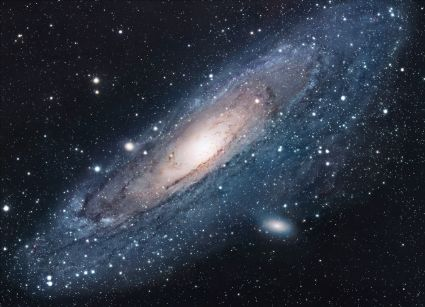
\includegraphics[scale=1.7]{universe.jpg}
%%\caption{The Universe}
%%\label{fig:univerise}
%\end{figure}
%``I always thought something was fundamentally wrong with the universe'' %\citep{adams1995hitchhiker}
